
% %%%%%%%%%%%%%%%%%%%%%%%%%%%%% TCC %%%%%%%%%%%%%%%%%%%%%%%%%%%%%%%%
% %
% % Template para TCC da 
% % Instituto Federal do Maranhão - campus Imperatriz
% %
% % Autor: Thiago Paiva Freire
% % Colaborador: Clovis Caface 
% %
% % Overleaf porting: Clovis Caface 
% % 
% % Revisão: Thiago Paiva Freire
% %          Clovis Caface
% %
% %%%%%%%%%%%%%%%%%%%%%%%%%%%%%%%%%%%%%%%%%%%%%%%%%%%%%%%%%%%%%%%%%%%

\documentclass{configuracoes}

% Alterar o arquivo a_dados_tcc.tex
%%%%%%%%%%%%%%%%%%%%%%%%%%%%%%%%%%%%%%%%%%%%%%%%%%%%%%%%%%%%%%%%%%%%%%%%%%%
% Inserir aqui os dados do trabalho a serem utilizados 
%%%%%%%%%%%%%%%%%%%%%%%%%%%%%%%%%%%%%%%%%%%%%%%%%%%%%%%%%%%%%%%%%%%%%%%%%%%

%%%%%%%%%%%%%%%%%%%%%%%%%%%%%%%
% Informações sobre localidade
%%%%%%%%%%%%%%%%%%%%%%%%%%%%%%%

% Cidade
\newcommand{\cidade}{Imperatriz}
% Estado 
\newcommand{\estado}{Maranhão}
% Sigla do estado
\newcommand{\siglaestado}{MA}

%%%%%%%%%%%%%%%%%%%%%%%%%%%%%%%%
% Informações sobre departamento
%%%%%%%%%%%%%%%%%%%%%%%%%%%%%%%%

\newcommand{\instituto}{Instituto Federal do Maranhão}

% digitar o nome do departamento (dep)
\newcommand{\dep}{Departamento de Ensino Superior e Tecnológico}

% sigla do departamento
\newcommand{\sigladep}{DESTEC}

%%%%%%%%%%%%%%%%%%%%%%%%%%%%%
% Informações sobre o curso 
%%%%%%%%%%%%%%%%%%%%%%%%%%%%%
% Titulacao do curso
\newcommand{\titulacao}{Bacharel}
% Nome do curso
\newcommand{\nomedocurso}{Ciência da Computação}

%%%%%%%%%%%%%%%%
% Sobre o autor
%%%%%%%%%%%%%%%%
% Nome do autor
\author{Autor}
% Titulo do trabalho
\title{Titulo}
% Subtitulo do trabalho
\newcommand{\subtitulo}{Subtitulo}
% \newcommand{\subtitulo}{} % quando não existir

%%%%%%%%%%%%%%
% Orientador 
%%%%%%%%%%%%%%
% Nome do Orientador
\renewcommand{\orientador}{Profº. Orientador}

% Orientador - comentar para alterar
\newcommand{\genorientador}{Orientador} % masculino
% \newcommand{\genorientador}{Orientadora} % feminino

% Coorientador - comentar para alterar
\renewcommand{\coorientador}{} % quando não existir
% \renewcommand{\coorientador}{Coorientador} % masculino
% \renewcommand{\coorientador}{Coorientadora} % feminino

% Nome do coorientador
\newcommand{\nomecoorientador}{} % deixar em branco quando não existir

%%%%%%%%%%%%%%%%%%%%%%%
% banca de examinadora
%%%%%%%%%%%%%%%%%%%%%%%
% Membros da Banca
\newcommand{\profb}{Membro da Banca 1}
\newcommand{\instprofb}{Instituto do Membro da Banca 1}

\newcommand{\profc}{Membro da Banca 2}
\newcommand{\instprofc}{Instituto do Membro da Banca 2}


\begin{document}
 \pretextual
 \begin{figure}[h]
\centering
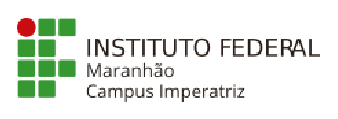
\includegraphics[scale=1.5]{imagens/logoifma.eps}
\end{figure}

\begin{center}
\MakeUppercase{\dep} \hspace*{2mm}- \sigladep \\
  \MakeUppercase{\nomedocurso}
\end{center}

  \vspace*{2in}
  \begin{center}
    \LARGE\textbf{ \thetitle:}\\
    \Large\textbf{ \subtitulo}\\
  \end{center}

  \vspace*{1in}

  \begin{center}
    {\MakeUppercase \theauthor}
  \end{center}

\vspace{2in}

\begin{center}
  \cidade \hspace*{2mm}- \siglaestado \\ \the\year
\end{center}


\begin{center}
  {\MakeUppercase \theauthor}
\end{center}

\vspace{3in}

\begin{center}
  {\huge \thetitle}\\
  \subtitulo
\end{center}

\vspace{1in}

\begin{flushright}
    \begin{minipage}{0.5\textwidth}
    Monografia apresentada ao curso \nomedocurso \hspace{1mm}do \dep, do \instituto, como requisito para a obtenção do grau de \titulacao \ em \nomedocurso
    \end{minipage}
    
    \vspace*{0.2in}
    
    \begin{minipage}{0.5\textwidth}
       \begin{minipage}[t]{0.35\textwidth}
        \genorientador
       \end{minipage}
       \begin{minipage}[t]{0.6\textwidth}
        \orientador
       \end{minipage}\\
       
       \begin{minipage}[t]{0.35\textwidth}
        \coorientador
       \end{minipage}
       \begin{minipage}[t]{0.6\textwidth}
        \nomecoorientador
       \end{minipage}
    \end{minipage}

\end{flushright}
\vspace*{.5in}

\begin{center}
    \Month \\ \the\year
\end{center} % Não necessita de alterações
 
 % Ficha Catalografica - necessita de alterações casuais, para mais informações acessar o arquivo 01_ficha_catalografica.tex
 % Isto é um exemplo de Ficha Catalográfica, ou ``Dados internacionais de
% catalogação-na-publicação''. Você pode utilizar este modelo como referência. 
% Porém, a biblioteca da universidade lhe fornecerá um PDF com a ficha catalográfica definitiva após a defesa do trabalho. Quando estiver com o documento, salve-o como PDF na pasta pdf do seu projeto e substitua todo o conteúdo de implementação deste arquivo pelo comando abaixo:

% \begin{fichacatalografica}
%     \includepdf{pdf/ficha_catalografica.pdf}
% \end{fichacatalografica}

% Comente ou retire todas as linhas abaixo após inserir o documento da ficha catalográfica

\begin{fichacatalografica}
	\sffamily
	\vspace*{2in}					% Posição vertical
    
	\begin{center}					% Minipage Centralizado
    	\fbox{
    	    \begin{minipage}[c][8cm]{13.5cm}		% Largura
            	\small
            	\imprimirautor
            	%Sobrenome, Nome do autor
            	
            	\hspace{0.5cm} \imprimirtitulo  / \imprimirautor. --
            	\cidade, \estado - 
            	
            	\hspace{0.5cm} \thelastpage p. : il. (algumas color.) ; 30 cm.\\
            	
            	\hspace{0.5cm} \genorientador~\orientador\\
            	
            	\hspace{0.5cm}
            	\parbox[t]{\textwidth}{Trabalho de Concluao de Curso~--~IFMA - Imperatriz/MA,
            	\Month de \the\year.}\\ 
            	
            	\hspace{0.5cm}
            		1. Palavra-chave1.
            		2. Palavra-chave2.
            		2. Palavra-chave3.
            		I. Orientador.
            		II. Universidade xxx.
            		III. Faculdade de xxx.
            		IV. Título 			
        	\end{minipage}
    	}
	\end{center}

\end{fichacatalografica}
 
 
 % Ficha de aprovação - necessita de alterações casuais, para mais informações acessar o arquivo 01_ficha_aprovação.tex
 \newpage
 
% Isto é um exemplo de Folha de aprovação, elemento obrigatório da NBR 14724/2011 (seção 4.2.1.3). Você pode utilizar este modelo até a aprovação do trabalho. Após isso, quando estiver com o documento com todas as assinaturas, salve-o como PDF na pasta pdf do seu projeto e substitua todo o conteúdo de implementação deste arquivo pelo comando abaixo:

% \begin{folhadeaprovacao}
% \includepdf{pdf/folhadeaprovacao_final.pdf}
% \end{folhadeaprovacao}

% Comente ou retire todas as linhas abaixo após inserir o documento da ficha de aprovação

\begin{folhadeaprovacao}

\begin{center}
\sigladep \hspace{2mm}- \dep \\
\instituto
\end{center}

\vspace{0.2in}

Trabalho de Conclusão de Curso de \nomedocurso \hspace*{0.1mm} intitulado \textit{\textbf{\em \thetitle}} de autoria de \theauthor, 
aprovada pela banca examinadora constituída pelos seguintes professores: 

\vspace{1in}

\begin{center}
 \begin{minipage}{0.6\textwidth}
  \hrule \vspace{0.05in}
  \orientador \\
  \genorientador\\
 \end{minipage}
  
  \vspace{1in}
 \begin{minipage}{0.6\textwidth}
  \hrule \vspace{0.05in}
  \profb\\
  \instprofb\\
 \end{minipage}
 
 \vspace{1in}
 \begin{minipage}{0.6\textwidth}
  \hrule \vspace{0.05in}
  \profc\\
  \instprofc\\
 \end{minipage}
\end{center}

\vfill

\begin{center}
\cidade, \today
\end{center}

\vspace{0.05in}

\newpage
\end{folhadeaprovacao}
 
 
 %Dedicatoria
 \section*{Dedicatória}
 \begin{dedicatoria}
    
    ***A dedicatória é opcional***
 % necessita de alterações
 \end{dedicatoria}
 
 %Agradecimentos
 \begin{agradecimentos}
    
    ***O agradecimento é opcional***
 % necessita de alterações
 \end{agradecimentos}
 
 
 %Epigrafe - comentar linha de baixo caso nao existe necessidade de epigrafe
 \begin{epigrafe}
    \vspace*{\fill}
	\begin{flushright}
	    
 *** A epígrafe é opcional ***
 % necessita de alterações
	\end{flushright}
 \end{epigrafe}
 
 \setlength{\absparsep}{18pt} % ajusta o espaçamento dos parágrafos do resumo
 \begin{resumo} % inserir resumo
    
Um resumo de trabalho de conclusão de curso é do tipo informativo e deve conter somente um parágrafo. A estrutura do resumo deve conter essencialmente os seguintes tópicos: apresentar inicialmente os objetivos do trabalho (o que foi feito?), a justificativa (porquê foi feito) e, finalmente, os resultados alcançados. O resumo deve informar ao leitor todas as informações importantes para o que o leitor possa entender o trabalho desenvolvido, quais foram as finalidades, a metodologia que o autor utilizou e os resultados obtidos. Deve conter frases curtas, porém completas (evitar estilo telegráfico); usar o tempo verbal no passado para os principais resultados e presente para comentários ou para salientar implicações significativas.  O resumo em português e inglês são obrigatórios e não devem passar de 200 palavras.

\textbf{ Palavras-chave:} \key{Primeira Palavra},  \key{segunda palavra}, \key{até 5 palavras}.

\key{Obs.: as palavras-chave devem ser escolhidas com bastante rigor, pois devem representar adequadamente os principais temas abordados pela pesquisa}.


 % necessita de alterações
 \end{resumo}
 
 \begin{resumo}[abstract] % inserir abstract
   \begin{otherlanguage*}{english}
     %Abstract%

A summary of paper is informative and should contain only one paragraph. The structure of the abstract should essentially contain the following topics: initially presenting the objectives of the paper (what was done?), The justification (why it was done) and, finally, the results achieved. The abstract should inform the reader of all the important information so that the reader can understand the paper developed, what were the purposes, the methodology that the author used and the results obtained. It should contain short but complete sentences (avoid telegraphic style); use verbal tense in the past for key results and present for comments or to point out meaningful implications. The abstract in Portuguese and English is mandatory and should not exceed 200 words.

\textbf{Key-words:} \key{First key}, \key{Second Key}, \key{until 5 keys}. % necessita de alterações, devem estar em ingles
   \end{otherlanguage*}
 \end{resumo}
 
 %Lista de figuras%
 \renewcommand{\listfigurename}{Lista de Figuras}
 \listoffigures
 
 \begin{siglas}
  \item[ABNT] Associação Brasileira de Normas Técnicas
  \item[abnTeX] ABsurdas Normas para TeX
  \item[IFMA]Instituto Federal do Maranhão
\end{siglas} % comentar caso nao seja usado, necessita alteração 

 \tableofcontents*
 \cleardoublepage

\textual
 % Introdução
 \chapter{INTRODUÇÃO}

Faça aqui, uma introdução geral da área do conhecimento à qual o tema escolhido está ligado. 

\section{Definição do Problema}

Dedique este tópico a esclarecer o que o pretende de fato com o seu esforço de pesquisa. Problema é a questão a ser respondida pelo trabalho, que motivou a sua realização. É uma questão que já tomou se formou em sua mente, derivada de teorias da área pesquisada e de sua observação sobre um fenômeno. Normalmente se utilizam os subitens abaixo como meios de se determinar claramente os objetivos, o que também colabora para a delimitação do escopo do trabalho. Está estreitamente ligado ao objetivo geral, que, normalmente, consiste em encontrar a resposta para o problema de pesquisa.

O que você viu que é um problema que precisa de solução? É viável? Você consegue fazer? O problema é sempre uma dificuldade, uma lacuna.

\subsection{Premissas e Hipóteses}
A melhor forma de determinar o tema abordado é através de premissas e hipóteses. A hipótese consiste em uma afirmativa que você considera verdadeira e que vai provar ou buscar provar ao longo de seu trabalho. Outra forma é delimitando o problema em forma de uma pergunta de partida. As hipóteses apresentadas aqui são provadas no seu trabalho é o que chamamos de tese. 

\subsubsection{Objetivo geral}
É a resposta ao problema especificado acima, ou seja, aquilo que se pretende fazer e que, depois de atingido, estará concluído o trabalho.. Alguns verbos utilizados para determinar o objetivo geral: contribuir / facilitar / subsidiar / propor / clarear / permitir / agregar / compreender.

\subsubsection{Objetivos específicos}
Os objetivos específicos detalham os objetivos gerais através de etapas ou fases de pesquisa. Devem ser utilizados verbos no infinitivo, assinalando as ações propostas para alcançar o objetivo geral. Os verbos utilizados aqui são os de ação, que serão utilizados na metodologia.

\subsection{Estrutura da monografia}
Neste item você vai descrever como está constituída a monografia, indicando o que será encontrado em cada uma das sessões seguintes.

 % necessita de alterações
 
 % Conceitos Gerais
 \chapter{CONCEITOS GERAIS E REVISÃO DA LITERATURA}

%Lembre-se que os capítulo, as sessões e sub-sessões são determinadas por si para adequar-se ao seu trabalho.

Neste capítulo deve ser proporcionado o estado da arte / referencial teórico sobre o tema a que se refere o estudo. Um bom pesquisador não deve repetir trabalhos já concluídos ou que já estão em andamento. Por isso esta sessão é onde o autor demonstra até onde vai a pesquisa atual no campo de estudos em questão e estabelece as bases sobre as quais desenvolverá o estudo proposto. 

\section{Conceitos Gerais}

\subsection{Exemplos de Objetos do Texto}

\subsubsection{Citações}
As citações em textos tal como \citeonline[p. 1]{examplephdthesis}, utilize o comando \textit{"citeonline"}, entre colchetes (opcional) está a referencia da página do trabalho, exemplo sem colchetes \citeonline{examplephdthesis}.

Citação em final de parágrafo utilize o comando cite. \cite{examplephdthesis}

O argumento (entre colchetes) também é opcional. \cite[p. 1]{examplephdthesis}

\subsubsection{Estruturas Matemáticas}
A seguir são mostrados alguns exemplos de como deve-se utilizar ambiente teorema, axioma, corolário, lema e demonstrações assim como inserir as figuras, citações diretas e tabelas. A Figura 01 mostra um exemplo de como inserir uma figura no texto. A Tabela 01 mostra o exemplo de como uma tabela deve ser inserida.

Para axiomas:
\begin{axm}[**Opcional o nome do axioma]
    Coisas que são iguais a uma mesma coisa, são iguais entre si.
\end{axm}

\begin{defi}[**Opicional o nome da definição]
A definição define o que deve ser definido.
\end{defi}

Para teoremas:
\begin{thm}[**Opcional o nome do teorema]
    \label{thm}
    Sejam $a, b$ os catetos e $c$ a hipotenusa de um triangulo retângulo, então $$ a^2+b^2=c^2$$
\end{thm}

Com sua demonstração
\begin{proof}
    Demonstração do teorema \ref{thm}, é trivial.
    
    \cqd % comando para inserir quadrado preto no fim da demonstração, se retirá-lo não aparecerá o quadrado preto.
\end{proof}

Para proposição:
\begin{prop}
Proposição é um termo usado em lógica para descrever o conteúdo de asserções. Uma asserção é um conteúdo que pode ser tomado como verdadeiro ou falso. Asserções são abstrações de sentenças não linguísticas que a constituem. A natureza das proposições é altamente controversa entre filósofos, muitos dos quais são céticos sobre a existência de proposições. Muitos lógicos preferem evitar o uso do termo proposição em favor de usar sentença
\end{prop}

Para corolários:
\begin{cor}[**Opcional o nome do corolário]
    \label{cor}
    Um corolário (do latim tardio corollarĭum) é uma afirmação deduzida de uma verdade já demonstrada. Assim como proposição resultante de uma verdade.
\end{cor}

Para lemas:
\begin{lem}[**Opcional o nome do lema]
    \label{lem}
    A palavra "lema" vem do grego $\lambda\acute{\eta}\mu\mu\alpha$ (lémma), no sentido de 'proposição'.
\end{lem}

\subsubsection{Equações}

Exemplo de equação com simbolo de integral
\begin{equation}
 \dint_{x=3}^{x=4} \dfrac{x^2+3}{x-a} \mbox{d}x
\end{equation}


Exemplo de como inserir equação por partes.
\begin{equation}
 f(x) = \left\{ 
 \begin{array}{ll}
  x^2+3x+1 & , x \geq 0 \\
  \ln |x^3|, x < 0
 \end{array}\right.
\end{equation}

Exemplo de contrução de matriz $3\times3$
\begin{equation}
  \left[
 \begin{array}{ccc}
  2 & 3 & 4 \\
  3 & 4 & 5 \\
  6 & 7 & 8 
 \end{array}
  \right]
\end{equation}

\subsection{Estruturas Textuais}
Para citação direta, teremos:
\begin{citacao}
	A Matemática é a chave do portão e as ciências. A falta de atenção às obras matemáticas prejudica todos os conhecimentos, uma vez que ele é ignorante de não poder conhecer as outras ciências ou as coisas deste mundo. \cite{exampleRogerCitacao}
\end{citacao}

\subsubsection{Figuras}
Para figuras:

\begin{figure}[h]
\centering
\caption{Exemplo de como inserir Figura}

\includegraphics[scale=0.75]{imagens/logo_latex.eps}
\label{fig:exemplo}
\fonte{acervo do texto-exemplo} 
\end{figure}

Referenciando a figura \ref{fig:exemplo} como se segue. Para inserir duas figuras será da seguinte forma:

\begin{figure}[h]
    \centering
    \caption{Imagens utilizadas}
    \begin{subfigure}[b]{0.3\textwidth}
        \centering
        \caption{Passarinho}
        
\includegraphics[scale=0.5]{imagens/logo_latex.eps}
        \label{fig:pas}
    \end{subfigure}
    \qquad
    \begin{subfigure}[b]{0.3\textwidth}
        \centering
        \caption{Brasão Universidade}
        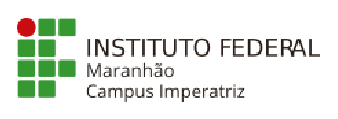
\includegraphics[scale=1]{imagens/logoifma.eps}
        \label{fig:uni}
    \end{subfigure}
    \fonte{acervo do texto-exemplo} 
    \label{fig:my_label}
\end{figure}

Podendo referenciar \ref{fig:pas} e \ref{fig:uni} como agora. Todas as imagens devem ser referenciadas, mesmo que sejam de autoria propria. Elas devem estar em extensão .EPS, para uma melhor visualização.

\subsubsection{Tabelas}

Para tabelas:
\begin{table}[h]
  \centering
  \caption{ Modelo de como as tabelas devem ser inseridas no texto }
  \begin{tabular}{|c|c|c|c|}
    \hline 
    \textbf {Índice} & \textbf{Coluna 01} &\textbf{ Coluna 02} & \textbf{Coluna 03} \\ \hline \hline
    Linha 01 & & & \\ \hline
    Linha 02 & & & \\ \hline                         
  \end{tabular}
  \fonte{Criação para o texto-exemplo} 
  \label{tab:modelo}
\end{table}


 % necessita de alterações
 
 % Metodologia
 \chapter{METODOLOGIA}
\section{Apresentação da Metodologia}
Aqui conterão os métodos e procedimentos adotados no desenvolvimento do trabalho. Esta é uma das sessões mais importantes pois demonstra o poder científico que foi utilizado para a pesquisa. Sem uma boa metodologia a pesquisa pode perder a validade. O pesquisador deve utilizar métodos ou técnicas aceitas pela comunidade científica na busca de provar suas hipóteses.

A metodologia escolhida deve ser aquela que mais se adéqua ao seu objeto de estudo e à abordagem aplicada. Há dois métodos principais: 1) quantitativo, que é o uso de instrumental estatístico, de dados numéricos; e 2) qualitativo, que se caracteriza pela qualificação dos dados coletados, durante a análise do problema.

 % necessita de alterações
 
 % Resultados
 \chapter{RESULTADOS}
Toda pesquisa deve apresentar uma análise sobre a investigação que foi realizada através da metodologia que foi aplicada. Nesta sessão é interessante inserir tabelas, gráficos, imagens que mostrem os resultados, análise de dados coletados, etc.

É interessante que nessa sessão o autor compare os seus resultados com os resultados de outros trabalhos existentes. Essa comparação aumenta a qualidade do trabalho e demonstra a relevância do mesmo. 

Nesta sessão o autor pode/deve incluir as contribuições científicas desenvolvidas tais como artigos, patentes, livros e outras contibuições que foram publicadas ou estão em fase de publicação e que são parte do trabalho.

 % necessita de alterações
 
 % Conclusao
 \chapter{CONCLUSÕES}
A conclusão deve conter os principais aspectos e contribuições de forma a finalizar o trabalho apresentado. Deve-se apresentar o que era esperado do trabalho através dos objetivos inseridos inicialmente e mostrar o que foi conseguido. 

	Não se deve inserir um novo assunto na conclusão. Aqui o autor apresentará as próprias impressões sobre o trabalho efetuado. 
    
É importante também que sejam identificadas limitações e problemas que surgiram durante o desenvolvimento do trabalho e quais as consequências do mesmo.

Os trabalhos futuros devem conter oportunidades de expansão do trabalho apresentado, bem como, novos projetos que puderam ser vislumbrados a partir do desenvolvimento do trabalho % necessita de alterações
 
 \postextual
 % Bibliografia
 \bibliography{b_referencias} % necessita de alterações
 
 % Inicia ambiente Apendice
 \begin{apendicesenv}
  
\chapter{Primeiro Apendice}

Teste de apendices

\section{Primeiro Subapendice}
 outro teste de Subapendice
\subsection{Primeiro subapendice}

\subsubsection{Primeiro subsubapendice}
 % necessita de alterações
 \end{apendicesenv}
 
 % Inicia ambiente Anexo
 \begin{anexosenv}
  

\chapter{Primeiro Anexo}
 % necessita de alterações
 \end{anexosenv}
 
\end{document}